\begin{comment}
%Heftig receiver clock error går fint fordi man går utifra at den er lik for alle satellitter til en gitt tid.
%Satellitposisjon oppgitt i ECEF men tar ikke høyde for jordrotasjonens innvirkning på pseudorange. Groves sier opptil 41m feil ved ekvator (Figur 7.5). Signalet er ikke følger ikke med jorda under transmission og blir feil. Bruk sagnac correction $\rho + \delta\rho_{ie, j}$. Bruker gjerne en tilnærming (ligning 7.27) fordi man tregner ECI-p_{si} og ECI-p.
%Jorda har rotert w_{ie}(t_{sa-t{st, j}) innen signalet ankommer fra satellitt j. Rotasjonsmatrise tilnærmes med small angle og (t_{sa-t{st, j}) = \rho_j/c

%Info
%farrel C.0:eq C.3: t_sv not reported.. t_sv = t_r - pr/c
%farrel C.1: t_sv og E_k coupled. Tilnærme t med t_sv går fint
%hvorfor ikke bare kepler? Farrel: The ephemeris parameters are the parameters for an extension of the orbital model predicted by Kepler. The extension is necessary to account for non-uniformities in the Earth gravitational field.
%GPS NAVSTAR: sqrt_A, C_rc og C_rs én meter sensitivitet, angular parameters 10^8 ig angular rate 10^12. Derfor bruke konstanter sånn de er oppgitt
%Doppler https://www.anacom.pt/streaming/PedroSilva_CongressoURSI2012.pdf?contentId=1148335&field=ATTACHED_FILE
%Hvis man har posisjonestimat når pseudorange kommer inn kan man sette lysfarten med hensyn på sagnac http://citeseerx.ist.psu.edu/viewdoc/download?doi=10.1.1.651.7591&rep=rep1&type=pdf
%Clock jump detection: http://citeseerx.ist.psu.edu/viewdoc/download?doi=10.1.1.833.4160&rep=rep1&type=pdf
%Ting som er vanskelig å finne andre steder: http://www.insidegnss.com/node/4505

\todo{Look over, rewrite, remove some parts}
\todo{Mention that GPS is looked at closer and exchange GPS with GNSS where applicable}
Although several satellite positioning systems exist, the following section focuses on the GPS as this was used in the experimental setup. Moreover, the terms GPS and GNSS may be used interchangeably.

\subsection{System structure}
\label{sec:sys_struct}
GNSS is split into three main \textit{segments}:

\begin{itemize}
\item Space segment: Composed of all satellite vehicles (SV) in orbit transmitting GNSS data.
\item Control segment: Monitors and updates the clock correction and orbital parameters of each satellite.
\item User segment: Composed of all GNSS-receivers. Both military, civilian and commercial.
\end{itemize}

Each GNSS satellite, hereby referred to as SV (satellite vehicle), in orbit contains three atomic clocks which are used to measure time with extreme precision. In addition each satellite frequently receives accurate estimates of its orbital parameters, also called the \textit{ephemeris}, which can be used to estimate the SV's position in space as a function of time (see section \ref{sec:ephemeris}). The orbital parameters and current time measured by the onboard atomic clocks are transmitted at given frequencies to the surface of the earth. Receivers may then measure the signals' time of flight to estimate the range between satellite and receiver by multiplying the measured time with the speed of light. In addition, data modulated on the given signal enables the receiver to calculate the satellites's position. The receiver's position can then be estimated through trilateration. See section \ref{sec:pos_det} for a more thorough explanation.\\

\todo{abbrev PRN}
\subsection{Signal composition}
For every SV to transmit distinguishable signals on the same frequency, a code, called a pseudorandom noise code (\textit{PRN}) is modulated onto the signal. These PRN codes have the interesting property that they are nearly orthogonal to each other, meaning that the cross correlation between two distinct PRN codes is low, while the autocorrelation peaks for a perfectly aligned signal. In this way, all SV's can transmit on the same frequency without risk of interfering with each other, although other sources of interference exist (see section \ref{sec:multipath}).

\subsubsection{Navigation signals}
Originally, only two signals were employed by the GPS:
\begin{itemize}
\item L1: 1575.42 MHz. Coarse acquisition code used by civilian receivers.
\item L2: 1227.60 MHz. Encrypted signal that can be used to employ extra ionospheric corrections, thereby improving accuracy.
\end{itemize}

Mathematically the two signals can be described, \cite{rep:Vik}:
\begin{align*}
	L_1(t) &= A_1P(t)D(t)cos(2\pi f_1t) + A_1C(t)D(t)sin(2\pi f_1t)\\
    L_2(t) &= A_2P(t)D(t)sin(2\pi f_2t)
\end{align*}
Where D(t) is the data payload at time t, $A_1$ and $A_2$ are the signal amplitudes and $f_1$ and $f_2$ are the L1 and L2 frequencies respectively. P(t) and C(t) are two PRN sequences of different length known as the \textit{precision} code, used by US military receivers, and the \textit{Coarse/Acquisition} code used by civilian receivers.\\

As the demand for precision GNSS is ever-increasing, the GPS is now in the process of being expanded with new and improved signals in addition to L1 and L2. It should be noted that the following have yet to become fully operational, however, although numerous functional SV's currently support them. They are mentioned here for the sake of completeness:

\begin{itemize}
\item L1C: An additional signal on the L1 frequency for enabling interoperability between GPS and other GNSS's.
\item L2C: New civilian signal on the L2 frequency for more accurate results in dual frequency receivers
\item L5: High powered signal intended to be used for aviation safety services. Using L5 in combination with L1 and L2C is expected to enable sub-meter accuracy in a single receiver, \cite{site:gps_signals}
\item M: New military signal intended for directed use at specifiable locations.
\end{itemize}

\subsubsection{Receiver structure} \todo{fjerne?}
Every receiver has an antenna tuned into the L1, and possibly L2, frequencies, a stable oscillator and a number of channels. The number of channels determines how many satellites can be tracked simultaneously, although they are carrier-frequency specific. In other words, to track both the L1 and L2 signals of a single satellite, two channels are needed. To lock on to a certain satellite,  the receiver assigns its known PRN code to a channel. The channel then performs a search along time and frequency to align the satellite's incoming PRN code with a replica. The satellite parameters modulated on the signal are then read and transmission time is calculated.


\subsection{Data structure}
\label{sec:data_types}
\todo{Time of week, gps week}
A full GPS message is grouped into 25 distinct \textit{frames} of 150 bit data each. The frames are in turn split into 300 bit \textit{subframes}, composed of ten 30 bit \textit{words}, as shown in figure \ref{fig:msg_struct}. The subframes all contain the same preamble of two words given by the telemetry word, TLM, and the handover word, HOW. The telemetry word contains a bit string for syncing purposes, while the HOW contains the current subframe ID, an anti-spoof status flag, data accuracy status flag and a truncated time of transmission to aid in rapid ground lock on, \cite[p.~42]{spec:gps}. The eight subsequent words contain information needed by the user to accurately calculate satellite position.\\

\begin{figure}[!htbp]
	\hspace{-1.5cm}
	\includegraphics[scale=0.5]{bilder/msg_struct.jpg}
    \caption{Message structure}
    \label{fig:msg_struct}
\end{figure}
%Time in the GPS is measured by week number and the seconds since the beginning of that week, \\

The subframe specific payloads can in short be summarized:
\begin{itemize}
	\item \textbf{Subframe 1}: Clock correction, GPS week count
	\item \textbf{Subframe 2}: Ephemeris
	\item \textbf{Subframe 3}: Ephemeris
	\item \textbf{Subframe 4}: Ionospheric model parameters, almanac
	\item \textbf{Subframe 5}: Almanac
\end{itemize}

\subsubsection{Ephemeris and clock correction}
\label{sec:ephemeris}
As mentioned in section \ref{sec:sys_struct}, the GPS is simply put a sophisticated time keeping system. To infer a receiver's position, it is however not only necessary to know the range between satellite and receiver but also the surrounding satellites' position. This is exactly what the ephemeris is for. The control segment updates each SV's ephemeris regularly by closely monitoring their position and movement through the sky from different points of the earth. After reporting the results to a master station, the ephemerides are in turn calculated through curve fitting\cite{farrell2008aided}, and uploaded to each SV. By applying each of the SV ephemerides to the ephemeris equations, satellite position can be calculated by a receiver as a function of time. The ephemerides and clock correction parameters are under normal conditions prescribed for four hour use, although the ephemeris is updated every hour \cite{spec:gps}, after which the old parameters are considered invalid. This stems from the fact that the orbital model is based on short term curve fitting to data points measured by the base stations of the control segment. The error being induced from this approach is further explained in section \ref{sec:eph_error}. To detect ephemeris updates, subframes 1, 2 and 3 each keep an issue of data variable that are all equal for a given ephemeris, but changes between ephemeris updates.\\

The ephemeris and clock correction parameters as well as the accompanying equations are shown in table \ref{tab:ephemeris} and equation set \ref{eq:ephemeris}, respectively. Additionally, figure \ref{fig:gps_ephemeris_block} shows a block diagram of the equations.\\
\subsubsection{Ephemeris equations}
\todo{Move to appendix}
\label{sec:eph_equations}
\begin{table}[!htbp]
\noindent
\textbf{Time}\\
\begin{tabular}{l r}
	\begin{tabular}{l | r}
	\multicolumn{2}{l}{\textit{Parameters}}\\
	\hline
	$t_{sv}$ & Satellite broadcast time \\
	$w_n$ & Satellite week \\
	$t_{ow}$ & Seconds in GPS week \\
	$t_{gd}$ & Group delay \\
    $t_{oc}$ & Clock data reference time \\
    $t_{oe}$ & Ephemeris reference time
	\end{tabular}
	&
	\begin{tabular}{l | r}
	\multicolumn{2}{l}{\textit{Corrections}}\\
	\hline
	$a_{f2}$ & Satellite clock correction 2 \\
	$a_{f1}$ & Satellite clock correction 1 \\
	$a_{f0}$ & Satellite clock correction 0 \\
	\multicolumn{2}{l}{}\\
	\multicolumn{2}{l}{}\\
    \multicolumn{2}{l}{}\\
	\end{tabular}
\end{tabular} \\

\vspace{0.5cm}
\noindent
\textbf{Orbital}\\
\begin{tabular}{l r}
	\begin{tabular}{l | r}
	\multicolumn{2}{l}{\textit{Parameters}}\\
	\hline
	$M_0$ & Mean anomaly at reference time\\
    $i_0$ & Inclination angle at reference time\\
    $\Omega_0$ & Longitude of ascending node of orbit\\
    $\omega$ & Argument of perigee\\
    e & Eccentricity\\
    $\sqrt{A}$ & Square root of semi-major axis\\
    $\dot{\Omega}$ & Rate of right ascension\\
    $\dot{i}$ & Rate of inclination angle \\
    
    
	\end{tabular}
	&
	\begin{tabular}{l | r}
	\multicolumn{2}{l}{\textit{Corrections}}\\
	\hline
	$C_{us}$ & Lateral correction \\
	$C_{uc}$ & parameters\\
	$C_{rc}$ & Radius correction \\
    $C_{rs}$ & parameters\\
	$C_{is}$ & Inclination correction\\
	$C_{ic}$ & parameters\\
    $\Delta n$ & Mean motion difference \\
    \multicolumn{2}{l}{}
	\end{tabular}
\end{tabular}

\vspace{0.5cm}
\noindent
\textbf{Validity}\\
\begin{tabular}{l | r}
	\multicolumn{2}{l}{\textit{Validity}}\\
	\hline
	IODC & Clock data validity \\
    IODE & Ephemeris validity\\
\end{tabular}
\caption{Ephemeris data}
\label{tab:ephemeris}
\end{table}

Several parameters are needed to calculate clock error and satellite position. Here as shown in \cite{farrell2008aided} and \cite{groves2013principles}. All of the parameters from the ephemerides are underlined.\\

\todo{Move to appendix?}
\missingfigure{Replace this with something better}
\begin{figure}[!htbp]
	\centering
	\includegraphics[scale=0.55]{bilder/GPS_equations_with_sub.png}
    \caption[Block diagram of ephemeris equations]{Block diagram of ephemeris equations resulting in satellite position in the ECEF frame}
    \label{fig:gps_ephemeris_block}
\end{figure}
\begin{subequations}
	\label{eq:ephemeris}
	\begin{align}
		\intertext{The measured satellite broadcast time contains small errors due to satellite clock bias and relativistic effects. The first step is therefore to apply the correction}		
        \Delta t_{sv} &= \underline{a_{f0}} + \underline{a_{f1}}(t - \bm{t_{oc}}) + \underline{a_{f2}}(t - \underline{t_{oc}})^2 + \Delta t_r\label{eq:eph_time_corr}\\
		\intertext{Where the relativistic correction $\Delta t_r$ is}
		\Delta t_r &= F\underline{e}\underline{\sqrt{A}}sin(E)\\
        \intertext{Where $F = -4.442807633E^{-10}$ is a constant and $E$ is calculated in equation \ref{eq:eph_ecc_anomaly}}
        \intertext{and the corrected satellite time is}
       	t &= t_{sv} - \Delta t_{sv} \label{eq:eph_corr_time}\\
        \intertext{Note that equation \ref{eq:eph_time_corr} and \ref{eq:eph_corr_time} are coupled. However, it has been found that $t_{sv}$ can approximate $t$ in this case without any notable lack in precision \cite{groves2013principles}.}
		\intertext{The mean motion is then computed as $n_0 = \sqrt{\frac{\mu}{\underline{A^3}}}$ and corrected}
		n &= n_0 + \underline{\Delta n}\\
        \intertext{With the time of signal transmission relative to the ephemeris reference time}
        \Delta t &= t_{st} - \underline{t_{oe}}
		\intertext{Mean anomaly, M, is then found}
		M &= \underline{M_0} + \bigg(n_0 + \underline{\Delta n}\bigg)\Delta t\\
        \intertext{To find the eccentric anomaly, $E$, Kepler's equation is solved iteratively}
        M &= E_k - \underline{e_0}sin(E_k)\\
        \label{eq:eph_ecc_anomaly}\nonumber
        \intertext{Performing 20 iterations should give centmetric accuracy, while 22 iterations yields millimetric accuracy \cite{groves2013principles}.}\nonumber
        \intertext{From the eccentric anomaly, the true anomaly can be found}
        \nu &= tan^{-1}\bigg(\frac{\sqrt{1-\underline{e_0}^2} sin(E)}{cos(E)-\underline{e_0}}\bigg)\\
        \intertext{Expressing position in polar coordinates, the argument of latitude is found as}
        \phi &= \underline{\omega} + \nu\\
        \intertext{The orbital radius varies with the eccentric anomaly however, harmonic perturbations are present here and in the argument of latitude as well as the inclination. Thus, the corrections of argument, radius and inclination, respectively, is found}
        \delta u &= \underline{C_{us}} sin(2\phi) + \underline{C_{uc}} cos(2\phi)\\
        \delta r &= \underline{C_{rs}} sin(2\phi) + \underline{C_{rc}} cos(2\phi)\\
      	\delta i &= \underline{C_{is}} sin(2\phi) + \underline{C_{ic}} cos(2\phi)\\
        \intertext{Applying these yields the corrected expressions}
        u &= \phi + \delta u\\
        r &= \underline{A}(1-\underline{e_0} cos(E)) + \delta r\\
        i &= \underline{i_0} + \delta i + \underline{\dot{i}}t\\
        \intertext{The transmitted longitude of the ascending node, $\underline{\Omega_0}$, is transmitted with respect to the week epoch. With respect to the reference time this is given by}
        \Omega &= \underline{\Omega_0} - w_{ie}(\Delta t + \underline{t_{oe}}) + \underline{\dot{\Omega}}\Delta t\\
        \intertext{Where $w_{ie} = 7.2921151467E^{-5}$ is the rotation rate of the Earth. Satellite position in the orbital plane is then found as}
        X &= r cos(u)\\
        Y &= r sin(u)\\
        \intertext{Finally, satellite position in the ECEF frame is given by}
        x &= X cos(\Omega) - Y cos(i)sin(\Omega)\\
        y &= X sin(\Omega) + Y cos(i)cos(\Omega)\\
        z &= Y sin(i)
        \intertext{It should also be noted that the equations should handle week crossovers, as the GPS time will be reset at this point. This is done by adding $\pm 604800$ to the corrected GPS time so that it stays in the intervall $[0, 302400]$.}\nonumber
	\end{align}
\end{subequations}

\subsection{Position estimation}
\label{sec:pos_det}
To compute the position of a receiver, SV positions must be calculated from the broadcast ephemerides and the distance between SV's and the receiver must be known. A number of errors affect the measurements however and instead of measuring true range, the receiver is said to measure the \textit{pseudorange}: The true range distorted by a number of different effects. \\

The pseudorange between receiver and a satellite \textit{i} can be modeled \cite{farrell2008aided, grewal2007global, groves2013principles}.
\begin{align}
	\label{gps_eq:pseudo_range}
	\rho_i &= \underbrace{r_i}_\text{True range} +
    		 \underbrace{\beta}_\text{Receiver clock error} +
             \underbrace{\varepsilon_i}_\text{User range error}
	\intertext{With} 
    r_i &= \sqrt{(\bf{p_{s_i}} - \bf{p})^T(\bf{p_{s_i}} - \bf{p})}
    \label{eq:range}
    \intertext{Where \textbf{p} is the position of the receiver and $\mathbf{p_{s_i}}$ is the position of satellite \textit{i}. The user range error is a collection of all the error terms that will be explained in section \ref{sec:errors} and $\beta$ is the range error, in meters, arising from the receiver clock bias. The user range error may be corrected to some degree, in which case it is assumed to be zero, yielding the following expression for the pseudorange}\nonumber\\
    \rho_i &= \sqrt{(\bf{p_{s_i}} - \bf{p})^T(\bf{p_{s_i}} - \bf{p})} + \beta
    \label{eq:range_estimate}
\end{align}

In measuring receiver positions, three unknowns must be found and consequently three SV measurements are needed, as indicated by figure \ref{fig:gps_range_est}. However, as most receivers use a cheap crystal oscillator, the bias can reach the order of milliseconds, leading to errors of more than a hundred kilometers, resulting in an infeasible GPS solution. Therefore, the receiver clock bias must be estimated as well, and consequently an additional satellite is necessary. See section \ref{sec:recv_error}.\\

\begin{figure}[!htb]
	\centering
    \figtable{0.15}{bilder/gps_satellite_1.png}
	\figtable{0.15}{bilder/gps_satellite_2.png}
    \\
	\figtable{0.15}{bilder/gps_satellite_3.png}
    \figtable{0.15}{bilder/gps_satellite_4.png}
    \caption{Multiple satellite readings are needed to infer receiver position.}
    \label{fig:gps_range_est}
\end{figure}


\todo{Put in implementation?}
After correcting the pseudorange measurements with the estimated receiver clock error and the methods mentioned in section \ref{sec:errors}, the receiver position can be inferred from equation \ref{eq:range_estimate}. Note however that this equation is nonlinear with respect to the receiver position and that it is also coupled with the satellite position. Therefore, one common method of solving equation \ref{eq:range_estimate} is by linearizing with respect to receiver position and receiver clock bias \cite{farrell2008aided}, \cite{groves2013principles}.
\begin{align*}
	%\Delta\rho &= H\Delta\bf{x} \numberthis\\
	%\text{With } 
    \label{eq:geometric_matrix}
    \intertext{Setting the matrix}
    H &=
	\begin{bmatrix}    		
		\partialdiff{\bf{r_1}}{\bf{p}}\at{\bf{p_e}} & 1\\[6pt]
	    \partialdiff{\bf{r_2}}{\bf{p}}\at{\bf{p_e}} & 1\\
    	\vdots & \vdots\\
    	\partialdiff{\bf{r_n}}{\bf{p}}\at{\bf{p_e}} & 1\\
	\end{bmatrix}\\
    &= 
    \begin{bmatrix}    		
		\frac{x_e - x_1}{r_1} & \frac{y_e - y_1}{r_1} & \frac{z_e - z_1}{r_1} & 1\\[6pt]
	    \frac{x_e - x_2}{r_2} & \frac{y_e - y_2}{r_2} & \frac{z_e - z_2}{r_2} & 1\\
    	\vdots & \vdots & \vdots & \vdots\\
    	\frac{x_e - x_n}{r_n} & \frac{y_e - y_n}{r_n} & \frac{z_e - z_n}{r_n} & 1\\[6pt]
	\end{bmatrix}\numberthis\\ 
    \intertext{Yields the linearized equation}
    \boldsymbol{\Delta\hat{p}} &= \boldsymbol{H\Delta x}
\intertext{ Where 
$
\mathbf{p_e} = 
\begin{bmatrix}
	x_e & y_e & z_e\\
\end{bmatrix}
$ 
is the linearization point, 
$
\mathbf{p_i} = 
\begin{bmatrix}
	x_i & y_i & z_i\\
\end{bmatrix}
$
is the position of satellite i, $r_i$ is the geometric range between receiver and satellite i, 
$
\Delta\bf{x} =
\begin{bmatrix}
	\Delta\bf{p} & \Delta\bf{\beta}
\end{bmatrix}^T
$ is the linearized state vector and $\bm{\Delta\hat{p}}$ is the resulting receiver position estimate.
}
\end{align*}

\todo{Remove}
Note that this method requires the equation to be solved iteratively, but depending on the linearization point might well be solved in only one iteration \cite{farrell2008aided}.

\subsection{User range error}
\label{sec:errors}
User range errors can be divided into stochastic and systematic errors. The stochastic errors vary with receiver and environment and includes the multipath and receiver noise errors, while the systematic errors depend on the position of the receiver in relation to the SVs and include atmospheric, relativistic and ephemeris errors among others, as explained below. \\

%https://www.e-education.psu.edu/geog862/node/1715
From \cite{farrell2008aided, groves2013principles} the following typical error magnitudes are
found: \todo{typical understrek}
\todo{Finn verdier på nytt}
\begin{itemize}
\item Ionospheric delay: 7 - 10 m
\item Tropospheric delay: 2.5 - 30 m
\item Multipath error: 0.1 - 3 m
\item Satellite clock error: 0.3 m
\item Receiver clock error: $\sim10^5$m
\item Receiver noise: 0.1 - 0.7 m
\item Ephemeris error: - 2 m
\item Relativistic errors: - 8 m
\item Earth rotation during transmission (sagnac effect): - 20 - 40 m
\end{itemize}

The following sections describes the different errors in detail.\\

\subsubsection{Ionospheric error}
When the GPS signals are transmitted through the atmosphere, the GPS's assumption that the signals travel in a straight line at constant speed no longer holds. The change in signal speed is much more significant than the change the effect on the signal path \cite{farrell2008aided} and is represented by the refractive index:

\todo{remove refractive index}
\begin{equation*}
	\eta = \frac{c}{v}
\end{equation*}
Where c is the speed of light and v is the actual signal speed. When the refraction index of a medium vary with signal frequency the medium is said to be \textit{dispersive}.\\

To model the atmospheric delay the atmosphere is divided into two layers. The ionosphere is the section of the atmosphere between 50 and 1000 km from the surface of the earth, while the troposphere is the lower layer between receiver and the ionosphere. The magnitude of the atmospheric errors each vary with the SV elevation angle as the length of exposure through the atmosphere increases inversely with elevation angle \cite{farrell2008aided, groves2013principles}. This is due to the fact that a lower elevation angle results in a longer travel path and by extension a longer exposure to the warping effects of the atmosphere. Figure \ref{fig:signal_prop} demonstrates this.\\

\begin{figure}[!htbp]
	\centering
	\includegraphics[scale=0.7]{bilder/atmospheric_error.png}
    \caption[GPS signal propagation to Earth]{GPS signal propagation to Earth. $P^1$ and $P^2$ is the entry point of two distinct satellite signals, while $E^1$ and $E^2$ is the elevation angle of the satellites.}
    \label{fig:signal_prop}
\end{figure}

The ionospheric error is a result of free ions and positively charged molecules in the ionosphere. The level of ionization depends on solar activity, seasons and time-of-day which directly affects the speed and travel time of GPS-signals, thereby resulting in an error in the range measured at the receiver. There are several ways of combating this, however. One approach is to take advantage of the fact that the ionosphere is dispersive by using a dual-frequency receiver. The residual ionospheric error in a dual-frequency receiver is in the order of 0.1 m \cite{groves2013principles}, and is the main reason the GPS employs two frequencies. Most receivers only use the L1 frequency however and must estimate the error through a secondary receiver or by mathematical models, such as the NeQuick \cite{di1990analytical} or Klobuchar models \cite{klobuchar1987ionospheric}. The latter is used by the GPS, and the external parameters needed by the receiver is transmitted in the almanac, while also being a function of the receiver position, satellite azimuth and elevation. \\

\begin{figure}[!htbp]
	\centering
	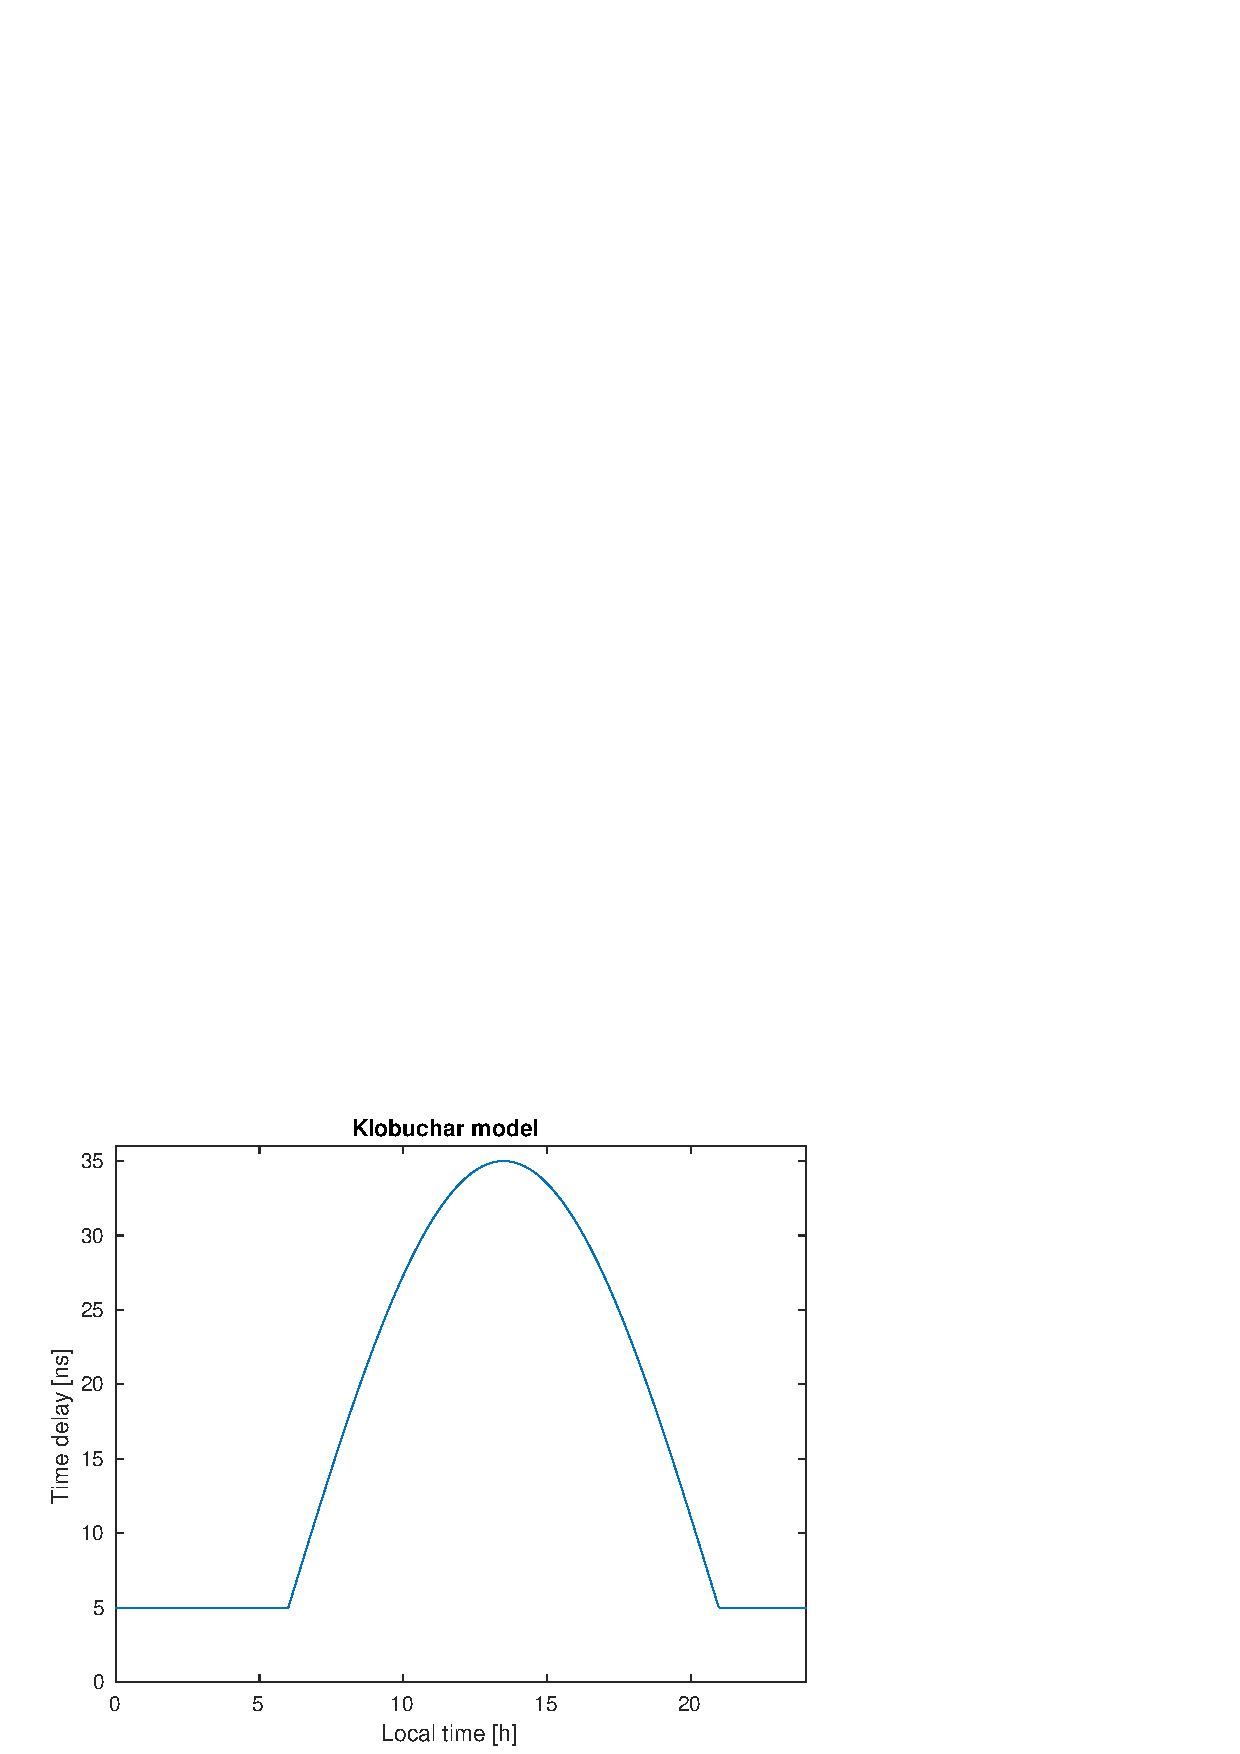
\includegraphics[scale=0.5]{bilder/klobuchar.png}
    \caption[Klobuchar model]{Klobuchar model (from \cite{site:navipedia})}
    \todo{Legg in i bibtex}
    \label{fig:klobuchar}
\end{figure}

\todo{make new figure?}
The Klobuchar model models ionospheric delay during daytime as a half cosine wave, while it is assumed constant at night. Figure \ref{fig:klobuchar} shows the Klobuchar model with time of day along the x-axis and ionospheric delay along the y-axis. Around 50\% of the total ionospheric delay is estimated to be corrected this way, \cite{farrell2008aided, groves2013principles, spec:gps}.\\

See the appendix \ref{sec:klobuchar} \todo{Add klobuchar to appendix}

\subsubsection{Tropospheric error}
The tropospheric error is usually the smallest of the atmospheric errors, but it is also much more sensitive to low elevation angles, with a worst case error of up to 30m\todo{verify 30 m}, \cite{farrell2008aided, groves2013principles}. As the troposphere is non-dispersive, delays are consistent for L1 and L2 and both single- and dual-frequency receivers must therefore rely on models to apply corrections. Normally, average values for the receiver's location is employed, although meteorological instruments can aid the receiver to obtain more precise results \cite{farrell2008aided}. \todo{Find example}\\

Gases like nitrogen and oxygen, normally called the dry components, and water vapor, called the wet component, affect the refraction index differently and must therefore be modeled separately. The dry components account for around 90\% of the tropospheric delay and is fairly easy to model as the parameters often are stable for a given area. The wet components are harder to model accurately as they are local and highly varying, but only accounts for about 10\% of the delay, \cite{farrell2008aided, groves2013principles}. For lower precision operations, the tropospheric delay can be simply modeled by elevation angle and user height alone, yielding a residual error of approximately $0.2 m$ \cite{groves2013principles}.\\

Typical ionospheric and tropospheric delays with respect to elevation angle is shown in figure \ref{fig:atmo_elev_error}.
\begin{figure}[!htbp]
	\centering
	\includegraphics[scale=0.5]{bilder/groves_elev_atmo_error.png}
    \caption[Relation between atmospheric errors and elevation]{Atmospheric errors as a function of satellite elevation angle. (From \cite{groves2013principles})}
    \label{fig:atmo_elev_error}
    \todo{Make new}
\end{figure}

\subsubsection{Multipath}
\label{sec:multipath}
Multipath errors occur when a satellite signal reach the receiver through multiple paths due to the signal reflecting off some surface. Signals that are reflected will arrive later than the signal taking the direct route and can usually be detected by the receiver if the delay is large enough. If the reflected signals arrive before the PRN code has been correlated however, interference can occur and shift the correlation peak. As the correlation peak is used to measure the delay from transmission to receival, pseudorange errors will occur. This also means that higher data rate signals are less susceptible to multipath errors, \cite{groves2013principles}. \todo{verify}\\

Signals from satellites at low elevations travel nearly parallel to the surface of the Earth and the chance of the signal being reflected off the ground is therefore substantially higher. Thus, discarding data from these satellites might improve the GPS solution, \cite{farrell2008aided}. \todo{additional sources needed or remove}

\subsubsection{Ephemeris error}
\label{sec:eph_error}
The ephemeris model is estimated through a curve fit to the measured orbit by the control segment and variations might therefore occur, \cite{farrell2008aided}. The result is a difference between actual and estimated SV position and the associated angle between actual and estimated signal path leads to a range error due to the long distance between receiver and SV. In fact, the sensitivity of position to the angular parameters in the ephemeris is in the order of $10^8 \deg$, while the angular rate parameters has a sensitivity in the order of $10^{12}deg/s$. \todo{citation needed}

\subsubsection{Satellite clock error}
Although the SV's use high precision atomic clocks, clock drift still occurs. To combat this the ephemeris keeps a precise estimate of this error in the form of a second degree polynomial which should be used to correct both raw pseudorange data and SV position estimates as described in section \ref{sec:ephemeris}.

\subsubsection{Receiver clock error}
\label{sec:recv_error}
As mentioned in section \ref{sec:pos_det}, the magnitude of the receiver clock error is significant and must be estimated by including an extra set of measurements. Figure \ref{fig:farrel_bias} shows how a typical receiver clock bias varies over time.\\
\todo{remove figure perhaps}
\begin{figure}[!htbp]
	\centering
	\includegraphics[scale=0.5]{bilder/farrel_bias.png}
    \caption{Typical receiver clock bias}
    \label{fig:farrel_bias}
\end{figure}

\todo{rewrite}
As the slope of the bias is constant, the receiver clock frequency does not match the nominal frequency exactly, although it is stable \cite{farrell2008aided}. The difference in frequency accumulates over time and many receivers accommodate this by periodically adding approximately one millisecond to its internal time scale. This can be seen as discontinuities of close to 300 km in the receiver clock bias and should be handled with care. %Kim et al \cite{art:Kim_et_al}, Heo et al \cite{art:Heo_et_al} and Guo et al \cite{art:Guo_et_al} look into ways of handling this. \todo{les disse}

\subsubsection{Relativistic errors} \todo{Fiks denne}
Due to the high speeds and different gravity potential of SV's, relativistic effects influences the SV clock frequencies. This can be split into a constant frequency component from the SV's nominal orbit, modified in factory, and a periodic frequency component due to the eccentricity of the orbit. The periodic component must be calculated by the receiver, as described in section \ref{sec:ephemeris}, and can lead to a navigation error of more than 8 m, \cite{art:Ashby}. \todo{check article and add to source or find new source}\\

Without the constant frequency correction applied, the difference in observed frequencies would accumulate to a clock error of approximately $38 \mu s$ a day, leading to a navigation error of 11 km, \cite{art:Ashby}\todo{check article and add to source or find new source}.

\subsubsection{Sagnac error}
As the ECEF frame is a rotating frame, the reference frame for satellite positions at transmission time will have rotated when the signal arrives. \todo{Improve. Add both approximation equations and rotation matrix}


\todo{Benefits of multi gnss}
\paragraph{Multi GNSS}
Several recievers supports multiple GNSS which can significantly improve the navigation solution by providing additional satellites and providing better constellation geometry \cite{li2017tightly}.


%For range error
% Først:    List over feilkilder med info
% Så:       Modell som inkluderer alle feil med ligninger
\end{comment}